\documentclass[a4paper]{article}

\usepackage[margin=2.5cm]{geometry}
\usepackage[pdftex]{graphicx}
\usepackage[utf8]{inputenc}
\usepackage[T1]{fontenc}
\usepackage{textcomp}
\usepackage{babel}
\usepackage{amsmath, amssymb}
\usepackage[colorlinks=true,linkcolor=blue]{hyperref}
\usepackage{float}
\usepackage{mathrsfs}
%\usepackage{enumitem}
%% for identity function 1:
\usepackage{bbm}
%%For category theory diagrams:
%\usepackage{tikz-cd}
%%For code (e.g. python) in latex:
%\usepackage{listings}
%
%Usage: 
%\begin{lstlisting}[language=Python]
%\end{lstlisting}

\newcommand{\incfig}[2][1]{%
\def\svgwidth{#1\columnwidth}
\import{./figures/}{#2.pdf_tex}
}


% figure support
\usepackage{import}
\usepackage{xifthen}
\pdfminorversion=7
\usepackage{pdfpages}
\usepackage{transparent}

\pdfsuppresswarningpagegroup=1

\setlength\parindent{0pt}

\newcommand{\qed}{\tag*{$\blacksquare$}}
\newcommand{\qedwhite}{\hfill \ensuremath{\Box}}

%Inequalities
\newcommand{\cycsum}{\sum_{\mathrm{cyc}}}
\newcommand{\symsum}{\sum_{\mathrm{sym}}}
\newcommand{\cycprod}{\prod_{\mathrm{cyc}}}
\newcommand{\symprod}{\prod_{\mathrm{sym}}}

%Linear Algebra

\DeclareMathOperator{\Span}{span}
\DeclareMathOperator{\Ima}{Im}
\DeclareMathOperator{\diag}{diag}
\DeclareMathOperator{\Ker}{Ker}
\DeclareMathOperator{\ob}{ob}
\DeclareMathOperator{\Hom}{Hom}
\DeclareMathOperator{\sk}{sk}


%Row operations
\newcommand{\elem}[1]{% elementary operations
\xrightarrow{\substack{#1}}%
}

\newcommand{\lelem}[1]{% elementary operations (left alignment)
\xrightarrow{\begin{subarray}{l}#1\end{subarray}}%
}

%SS
\DeclareMathOperator{\supp}{supp}
\DeclareMathOperator{\Var}{Var}

%NT
\DeclareMathOperator{\ord}{ord}

%Alg
\DeclareMathOperator{\Rad}{Rad}
\DeclareMathOperator{\Jac}{Jac}

\DeclareMathAlphabet{\pazocal}{OMS}{zplm}{m}{n}
\newcommand{\unif}{\pazocal{U}}

\begin{document}
    \textbf{1:}\\
    (a) We prove it by induction.\\
    Suppose $f = f_0$. Since $f$ is constant, if $f \left( \lambda a_1, \ldots
    , \lambda a_{n+1}\right) = 0$ for any $(a_1, \ldots, a_{n+1})$, then
    $f$ is identically zero. Hence $f_0 = f = 0$.\\
    Assume it is proved for all $d \le N$.\\
    Now assume
    $f \left( \lambda a_1, \ldots , \lambda a_{n+1} \right) = 0$ for all
    non-zero scalars $\lambda \in k$ and
    $f = f_0 + f_1 + \ldots + f_{N+1}$. 
    Then we have for each $f_i$ that
    \[
    f_i (\lambda a_1, \ldots, \lambda a_{n+1}) = \lambda^{i}
    f_i (a_1, \ldots, a_{n+1}),
    \] 
    so
    \begin{align*}
    c_0 + \left| \lambda \right| c_1 + \ldots +
     \left| \lambda \right|^{N} c_N
    &\geq \left| f_0 (a_1, \ldots, a_{n+1}) + 
    \lambda f_1 \left( a_1, \ldots, a_{n+1} \right) 
    + \ldots + \lambda^{N} f_{N}(a_1, \ldots, a_{n+1}) \right|\\
    &= \left| f_0 (\lambda a_1, \ldots, \lambda a_{n+1})
    + \ldots + f_N \left( \lambda a_1, \ldots, \lambda a_{n+1} \right) \right|
    \\
    &= \left| f_{N+1} \left( \lambda a_1, \ldots, \lambda a_{n+1} \right)
    \right|\\
    &= \left| \lambda \right|^{N+1} \left| f_{N+1}\left( a_1, \ldots, a_{n+1} \right)  \right| 
    = \left| \lambda \right|^{N+1} c_{N+1},
    \end{align*}
    where $c_i = \left| f_{i}(a_1, \ldots, a_{n+1}) \right| $.\\
    So in particular, for positive $\lambda$, we have
    \[
    c_0 + \lambda c_1 + \ldots + \lambda^{N} c_N \geq \lambda^{N+1} c_{N+1}
    \tag{$\zeta$}
    \] 
    
    Now assuming $c_{N+1} \neq 0$, choose
    \[
        \lambda = \frac{\left| c_0 \right| + \left| c_1 \right| 
        + \ldots + \left| c_{N} \right| }{\left| c_{N+1} \right| } + 1.
    \] 
    Note that $\lambda \ge 1$, and thus $\lambda^{j} \le \lambda^{N}$ for
    $j = 0, 1, \ldots, N$, so using the triangle inequality, we have
    \begin{align*}
        c_0 + \ldots + c_N \lambda^{N}
        &= \left| c_0 + c_1 \lambda + \ldots + c_N \lambda^{N} \right|\\
        &\le  \left( \left| c_0 \right| + \ldots + \left| c_N \right|  \right) 
        \lambda^{N}\\
        &< \left| c_{N+1} \lambda^{N+1} \right| 
        = c_{N+1} \lambda^{N+1},
    \end{align*}
    but this contradicts $(\zeta)$. Hence
    $0 = c_{N+1} = \left| f_{N+1}(a_1, \ldots, a_{n+1}) \right| $, so
    $f_{N+1} \left( a_1, \ldots, a_{n+1} \right) = 0$. Hence
    for all $\lambda \in k$,
    \begin{align*}
    0 = f\left( \lambda a_1 ,\ldots, \lambda a_{n+1} \right) 
    &= f_0 \left( \lambda a_1, \ldots, \lambda a_{n+1} \right) 
    + \ldots + f_N \left( \lambda a_1, \ldots, \lambda a_{n+1} \right) 
    + \underbrace{f_{N+1} \left( \lambda a_1 , \ldots , \lambda a_{n+1}
    \right)}_{= \lambda^{N+1} f\left( a_1, \ldots, a_{n+1} \right) =0}\\
    &= f_0 \left( \lambda a_1, \ldots, \lambda a_{n+1} \right) 
    + \ldots + f_N \left( \lambda a_1, \ldots, \lambda a_{n+1} \right).
    \end{align*}
    By the inductive assumption, we now get
    $f_i \left( a_1, \ldots, a_{n+1} \right) $ for all $i \in \left\{ 1,\ldots,
    N+1\right\} $, which gives the result by induction.\\
    \linebreak
    (b)  Suppose $Y \subset \mathbb{A}^{n+1}$ is a cone. Then
    for any $(x_1, \ldots, x_{n+1}) \in Y$, and for any $\lambda \in k$, we
    have
    $\left( \lambda x_1, \ldots, \lambda x_{n+1} \right) \in Y$, so
    assume $f \in I(Y)$ and $f = f_0 + f_1 + \ldots + f_d$. Choose
    any point $(a_1, \ldots, a_{n+1}) \in Y$. Then
    for all non-zero scalars $\lambda \in k$, we have
    $(\lambda a_1, \ldots, \lambda a_{n+1}) \in Y$, so
    \[
    f\left( \lambda a_1, \ldots, \lambda a_{n+1} \right), \quad \forall \lambda
    \in k,
    \] 
    so by (a), we have $f_i \left( a_1 , \ldots, a_{n+1} \right) = 0$ for all
    $i = 0,\ldots, d$, and as $(a_1, \ldots, a_{n+1}) \in Y$  was arbitrary, we
    have
    that for any $i \in \left\{ 0, \ldots, d \right\}$, 
    $f_i \in I(Y)$, so by past (2) of the last definition/proposition on lecture note 18,
    we
    have that $I(Y)$ is a homogeneous ideal.\\
    \linebreak
    \textbf{2:}\\
    (a) As  $U_1 = \left\{ \left[ x_1  \colon x_2  \colon x_3 \right] 
    \in \mathbb{P}^2  \colon x_1 \neq 0 \right\} $, we have
    that the complement is
    $L_1 = \left\{ \left[ 0  \colon x_2  \colon x_3 \right] \in \mathbb{P}^2
    \right\} $, and similarly,
    $L_2 = \left\{ \left[ x_1  \colon 0  \colon x_3 \right] \in \mathbb{P}^2 \right\} $ 
    and
    $L_3 = \left\{ \left[ x_1  \colon x_2  \colon 0 \right]  \in \mathbb{P}^2
    \right\} $. 
    Hence $L_1 \cap L_2 = 
    \left\{ \left[ x_1  \colon x_2  \colon x_3 \right] \in \mathbb{P}^2  \colon
    x_1 = 0 = x_2 \right\} =
    \left\{ \left[ 0  \colon 0  \colon x_3 \right] \in \mathbb{P}^2 \right\}
    = \left\{ \left[ 0:0:1 \right]  \right\} 
    $.
    Similarly,
    $L_1 \cap L_3 = \left\{ \left[ 0  \colon 1  \colon 0 \right] 
     \right\} $ and
    $L_2 \cap L_3 = \left\{ \left[ 1  \colon 0  \colon 0 \right]
     \right\} $.\\
     \begin{figure}[H]
         \centering
         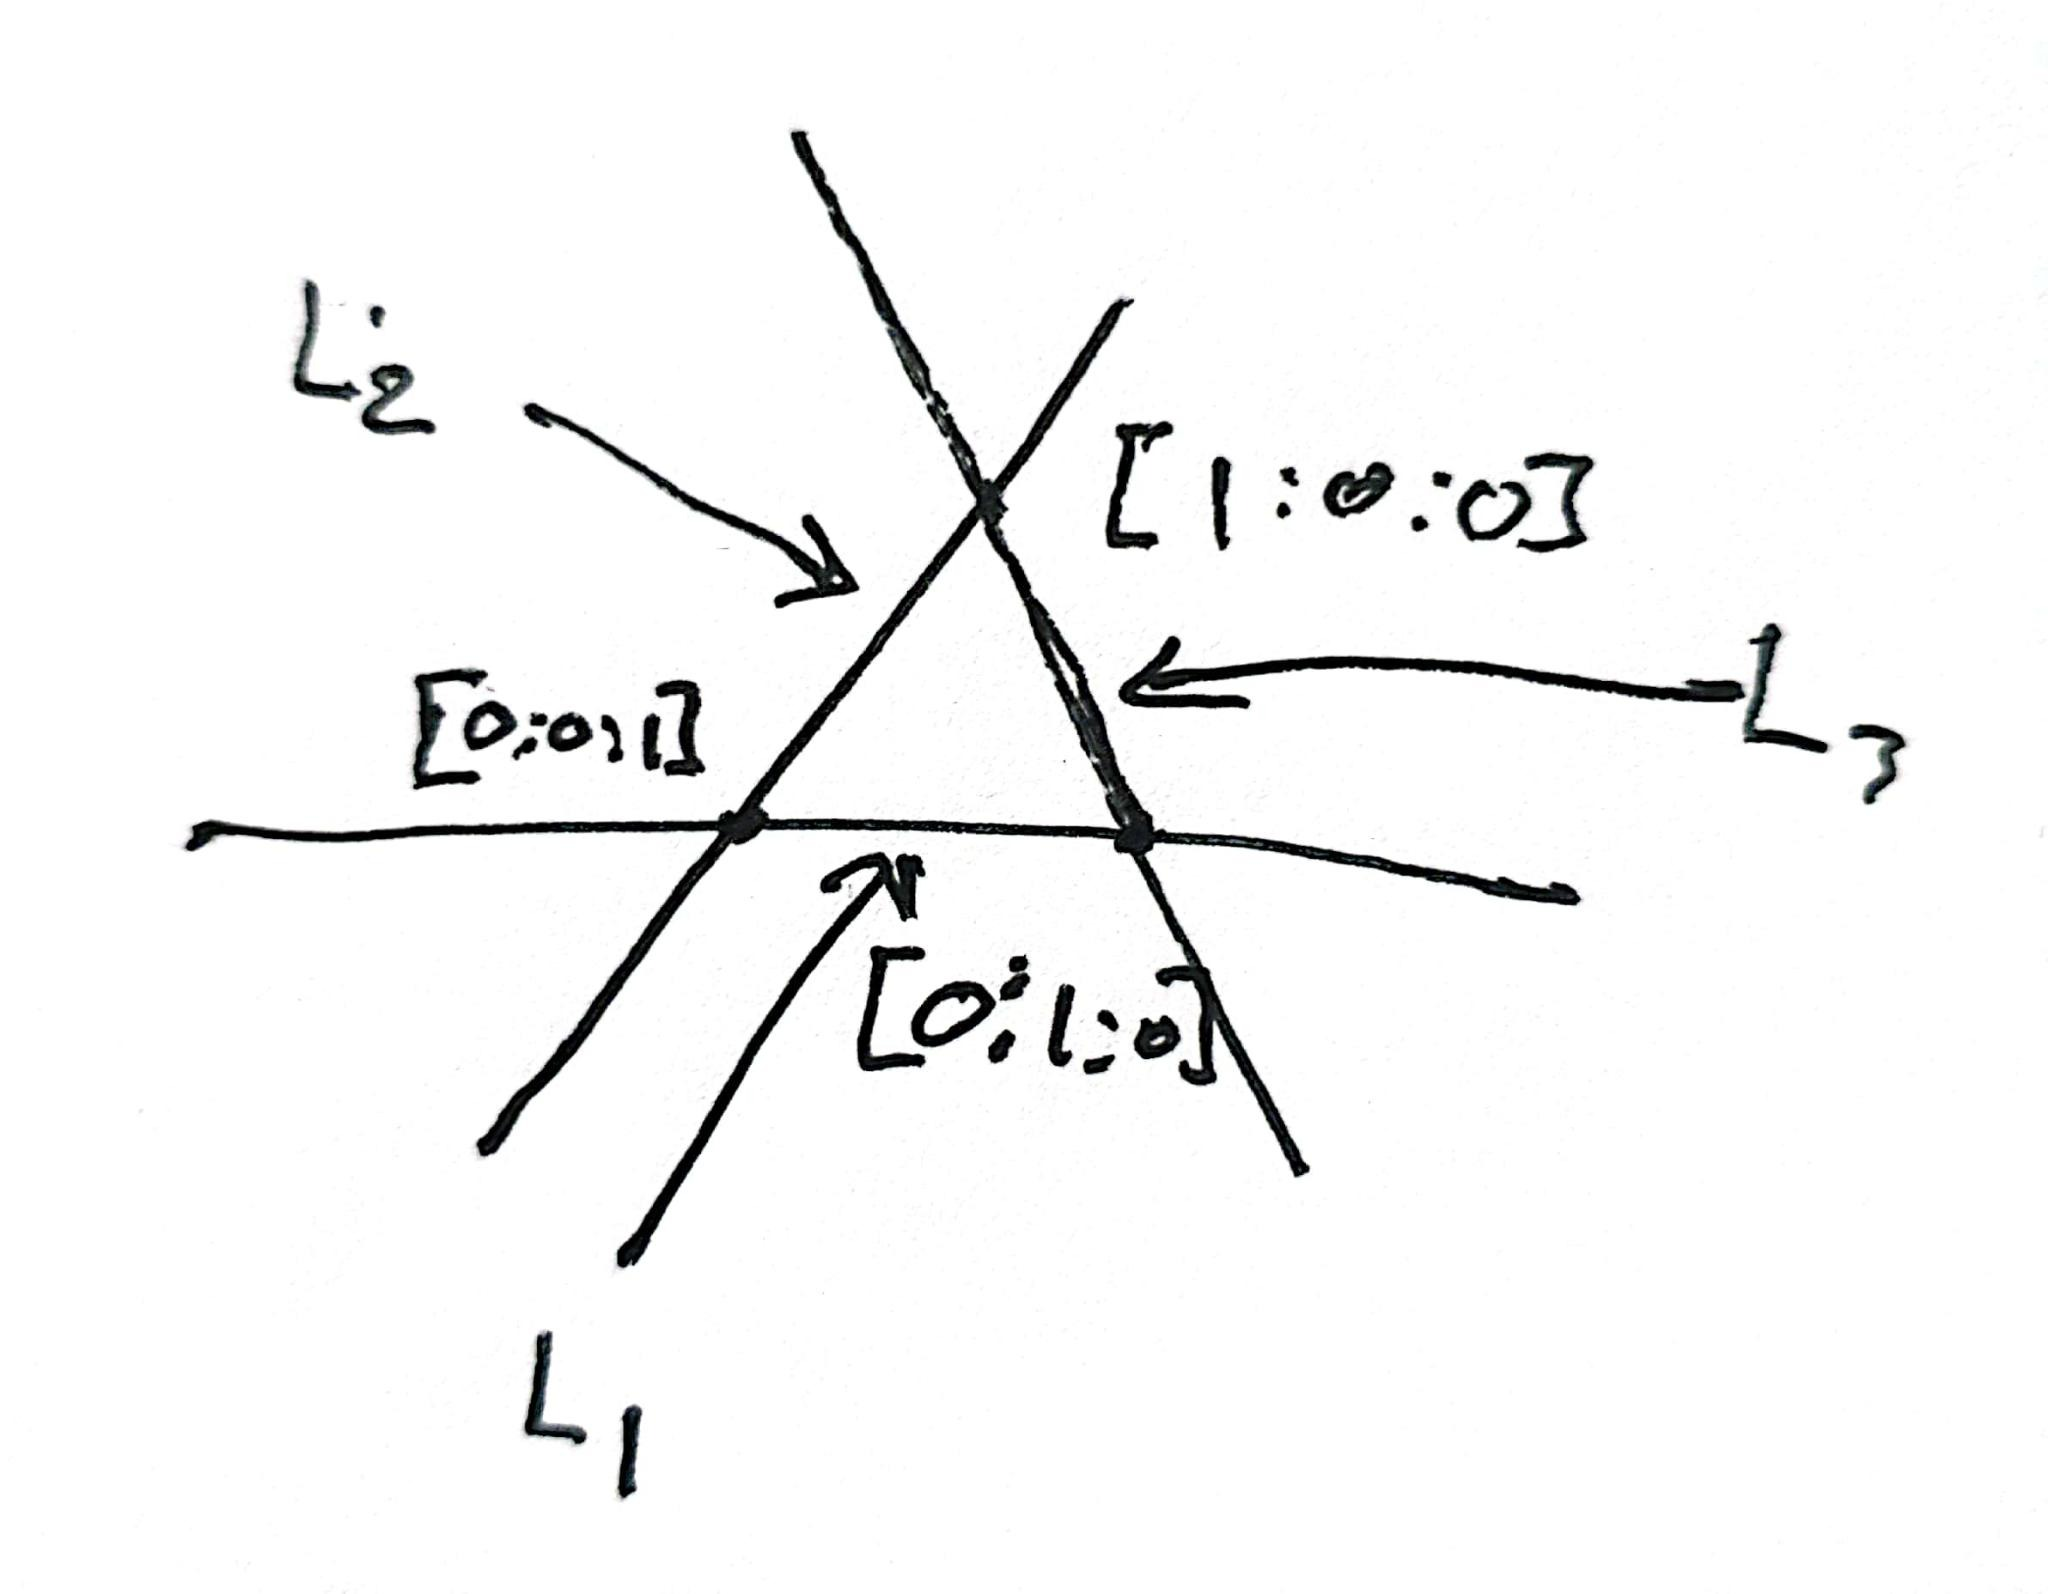
\includegraphics[width=0.6\textwidth]{2.jpeg}
         \label{fig:2-jpeg}
     \end{figure}
    (b) A point $\left[ x_1  \colon x_2  \colon x_3 \right] \in \mathbb{P}^2$ 
    is
    in $U_i$ if and only if $x_i \neq 0$, so it belongs to all three affine
    charts if and only if $x_1, x_2, x_3 \neq 0$, that is
    \[
    U_1 \cap U_2 \cap U_3 = \left\{ \left[ x_1  \colon x_2  \colon x_3 \right]
    \in \mathbb{P}^2  \colon x_1, x_2, x_3 \neq 0 \right\} .
    \] 
    (c) A point
    $\left[ x_1  \colon x_2  \colon x_3 \right] \in \mathbb{P}^2$ belongs to only one affine chart, say  $U_i$, if and only
    if  $x_i \neq 0$ and the remaining coordinates are $0$.\\
   So the point belongs to only $U_1$ for example, if 
   and only if
   $x_1 \neq 0$ and $x_2 = 0 = x_3$.\\
   \linebreak
   \textbf{3:} \\
   (a) The corresponding projective algebraic set in $\mathbb{P}^2$ 
   is $\left\{ \left[ x  \colon y  \colon 1 \right]  \colon
   x = y^2 \right\} =
   \left\{ \left[ x  \colon y  \colon z \right]  \colon
   z x = y^2 \right\} =
   \mathbb{V} \left( zx - y^2 \right) $ by homogenization.\\
   \linebreak
   (b) The intersection is
   \[
   \mathbb{V}(zx - y^2) \cap \mathbb{V}(z) =
   \left\{ \left[ x  \colon y  \colon z \right]  \in \mathbb{P}^2  \colon
   zx = y^2     \right\} \cap \left\{ \left[ x  \colon y  \colon 0 \right] \in
   \mathbb{P}^2 \right\} 
   = \left\{ \left[ x \colon y  \colon 0 \right]  \colon
   0 = y^2 \right\} =
   \left\{ \left[ x  \colon 0  \colon 0 \right] \in \mathbb{P}^2 \right\}.
   \] 
   (c) 
   We have
   \begin{align*}
       \mathbb{V}(zx - y^2) \cap U_1
       &= \left\{ \left[ x  \colon y  \colon z \right]  \colon
       zx = y^2 \right\} \cap \left\{ \left[ x \colon y  \colon z \right]  \colon
       x \neq  0 \right\} 
       = \left\{ \left[ x  \colon y  \colon z \right]  \colon
       zx = y^2 , x \neq 0 \right\}
       = V \left( z - y^2 \right) \\
       \mathbb{V}(zx - y^2) \cap U_2
       &= \left\{ \left[ x  \colon y  \colon z \right]  \colon
       zx = y^2 \right\} \cap \left\{ \left[ x \colon y  \colon z \right]  \colon
       y \neq  0 \right\} 
       = \left\{ \left[ x  \colon y  \colon z \right]  \colon
       zx = y^2 , y \neq 0 \right\}
       = V\left( zx - 1 \right) \\
       \mathbb{V}(zx - y^2) \cap U_3
       &= \left\{ \left[ x  \colon y  \colon z \right]  \colon
       zx = y^2 \right\} \cap \left\{ \left[ x \colon y  \colon z \right]  \colon
       z \neq  0 \right\} 
       = \left\{ \left[ x  \colon y  \colon z \right]  \colon
       zx = y^2 , z \neq 0 \right\}
       = V\left( x - y^2 \right) 
   \end{align*}
   Furthermore
   \begin{align*}
       \mathbb{V}(z) \cap U_1
       &= \left\{ \left[ x : y : 0 \right]  \right\} 
       \cap \left\{ \left[ x : y : z \right]  \colon x \neq 0 \right\} 
       = \left\{ \left[ x : y : 0 \right]  \colon x\neq 0 \right\}
       = \left\{ \left[ 1  : y: 0 \right]  \right\} \\
       \mathbb{V}(z) \cap U_2
       &= \left\{ \left[ x : y : 0 \right]  \right\} 
       \cap \left\{ \left[ x : y : z \right]  \colon y \neq 0 \right\} 
       = \left\{ \left[ x : y : 0 \right]  \colon y\neq 0 \right\}
       = \left\{ \left[ x : 1 : 0 \right]  \right\} \\
       \mathbb{V}(z) \cap U_3
       &= \left\{ \left[ x : y : 0 \right]  \right\} 
       \cap \left\{ \left[ x : y : z \right]  \colon x \neq 0 \right\} 
       = \varnothing
   \end{align*}

   \begin{figure}[H]
       \centering
       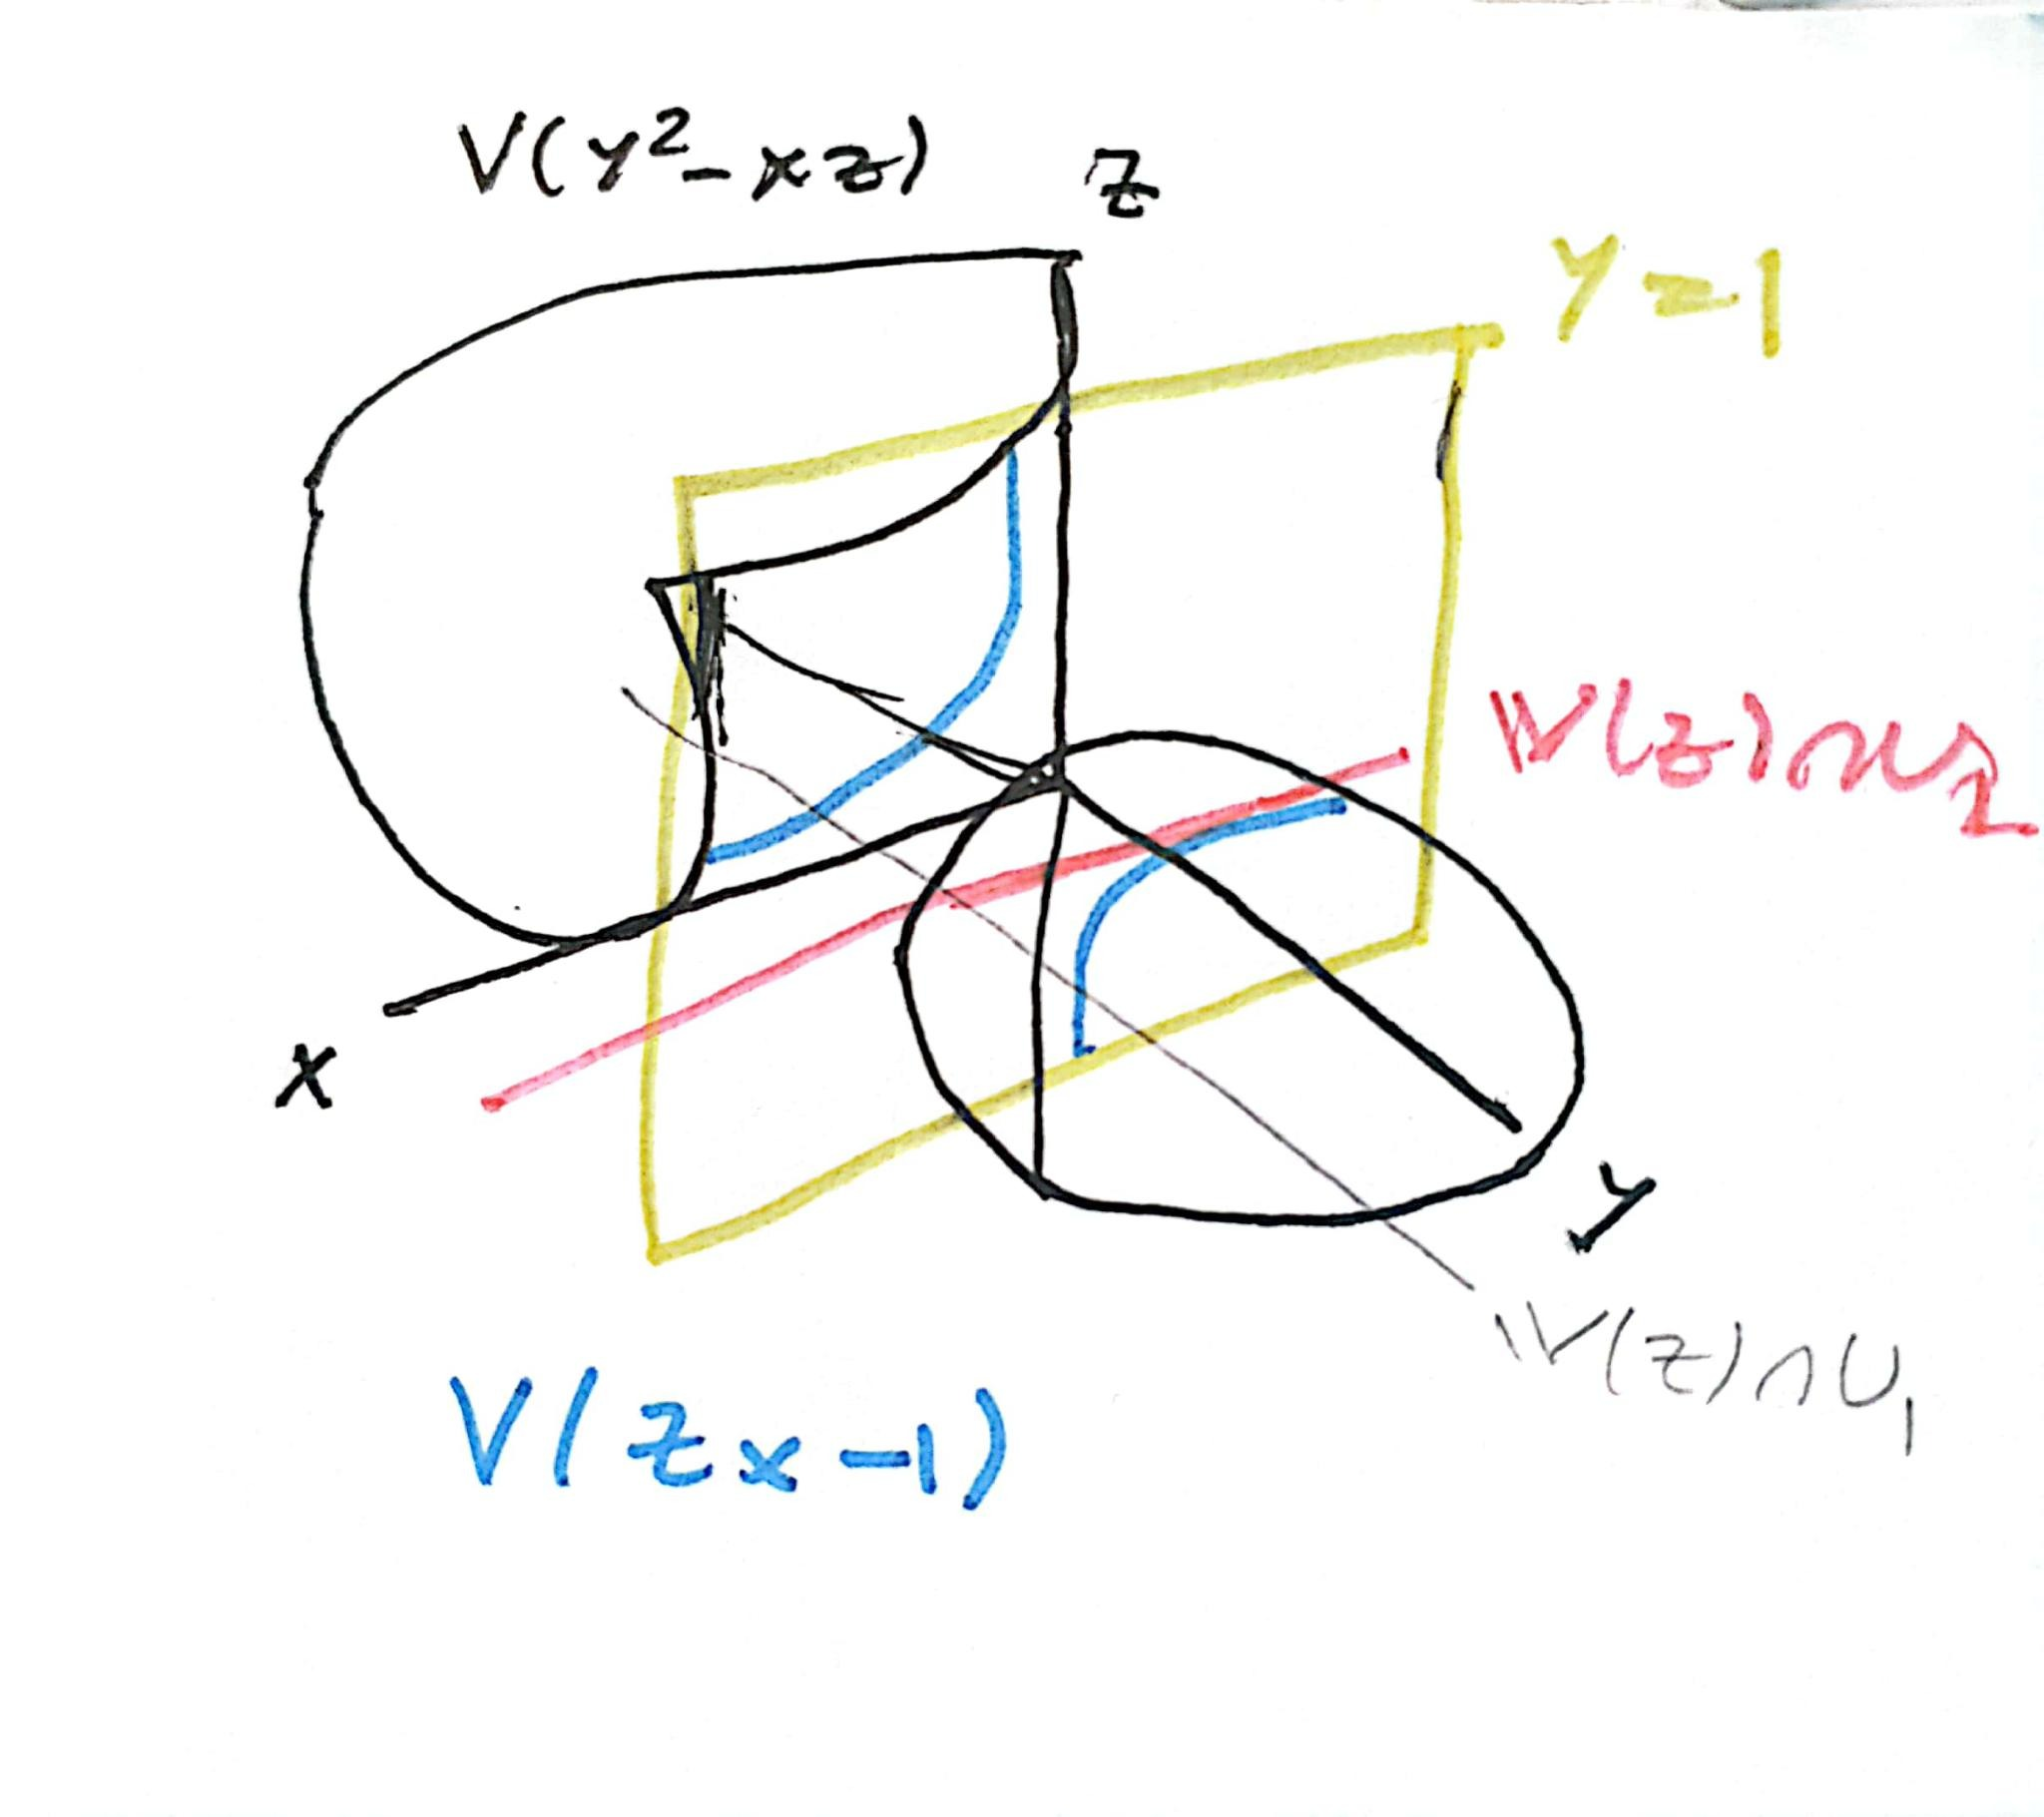
\includegraphics[width=0.8\textwidth]{3c2.jpeg}
       \label{fig:3c2-jpeg}
   \end{figure}
   \begin{figure}[H]
       \centering
       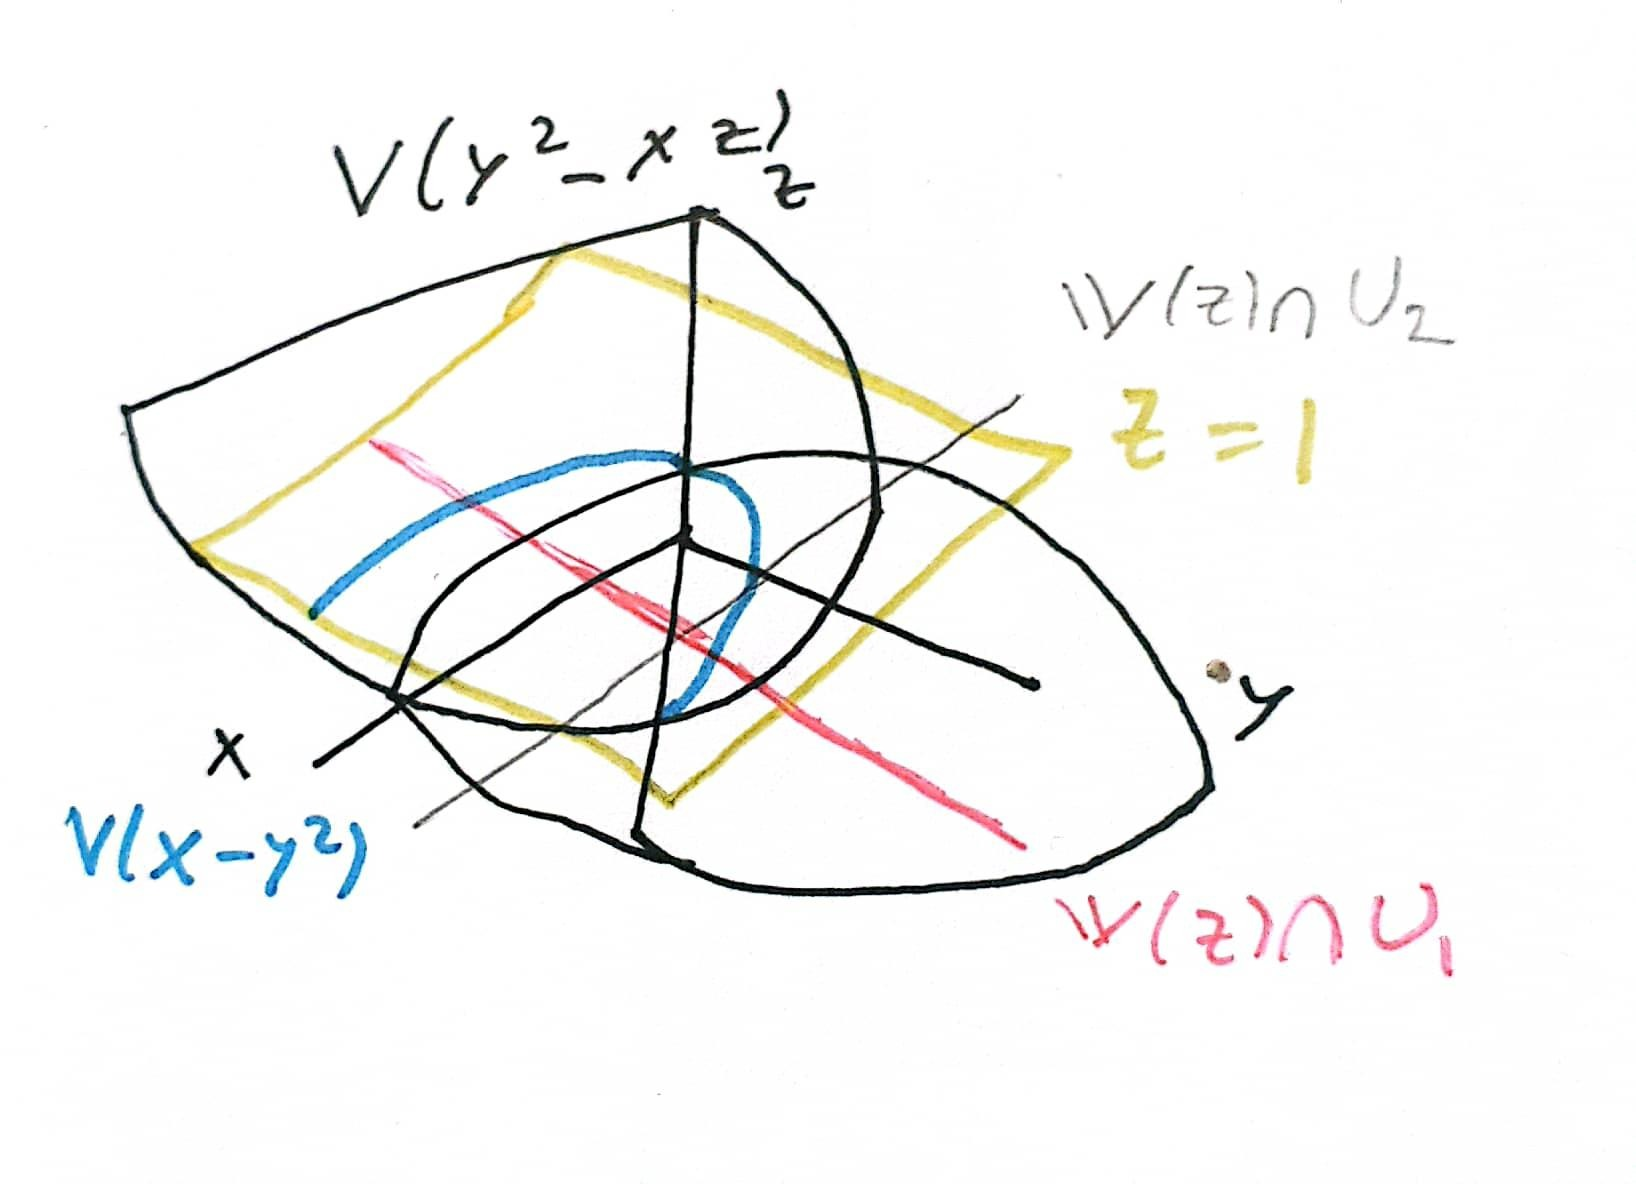
\includegraphics[width=0.8\textwidth]{3c3.jpeg}
       \label{fig:3c3-jpeg}
   \end{figure}
   \begin{figure}[H]
       \centering
       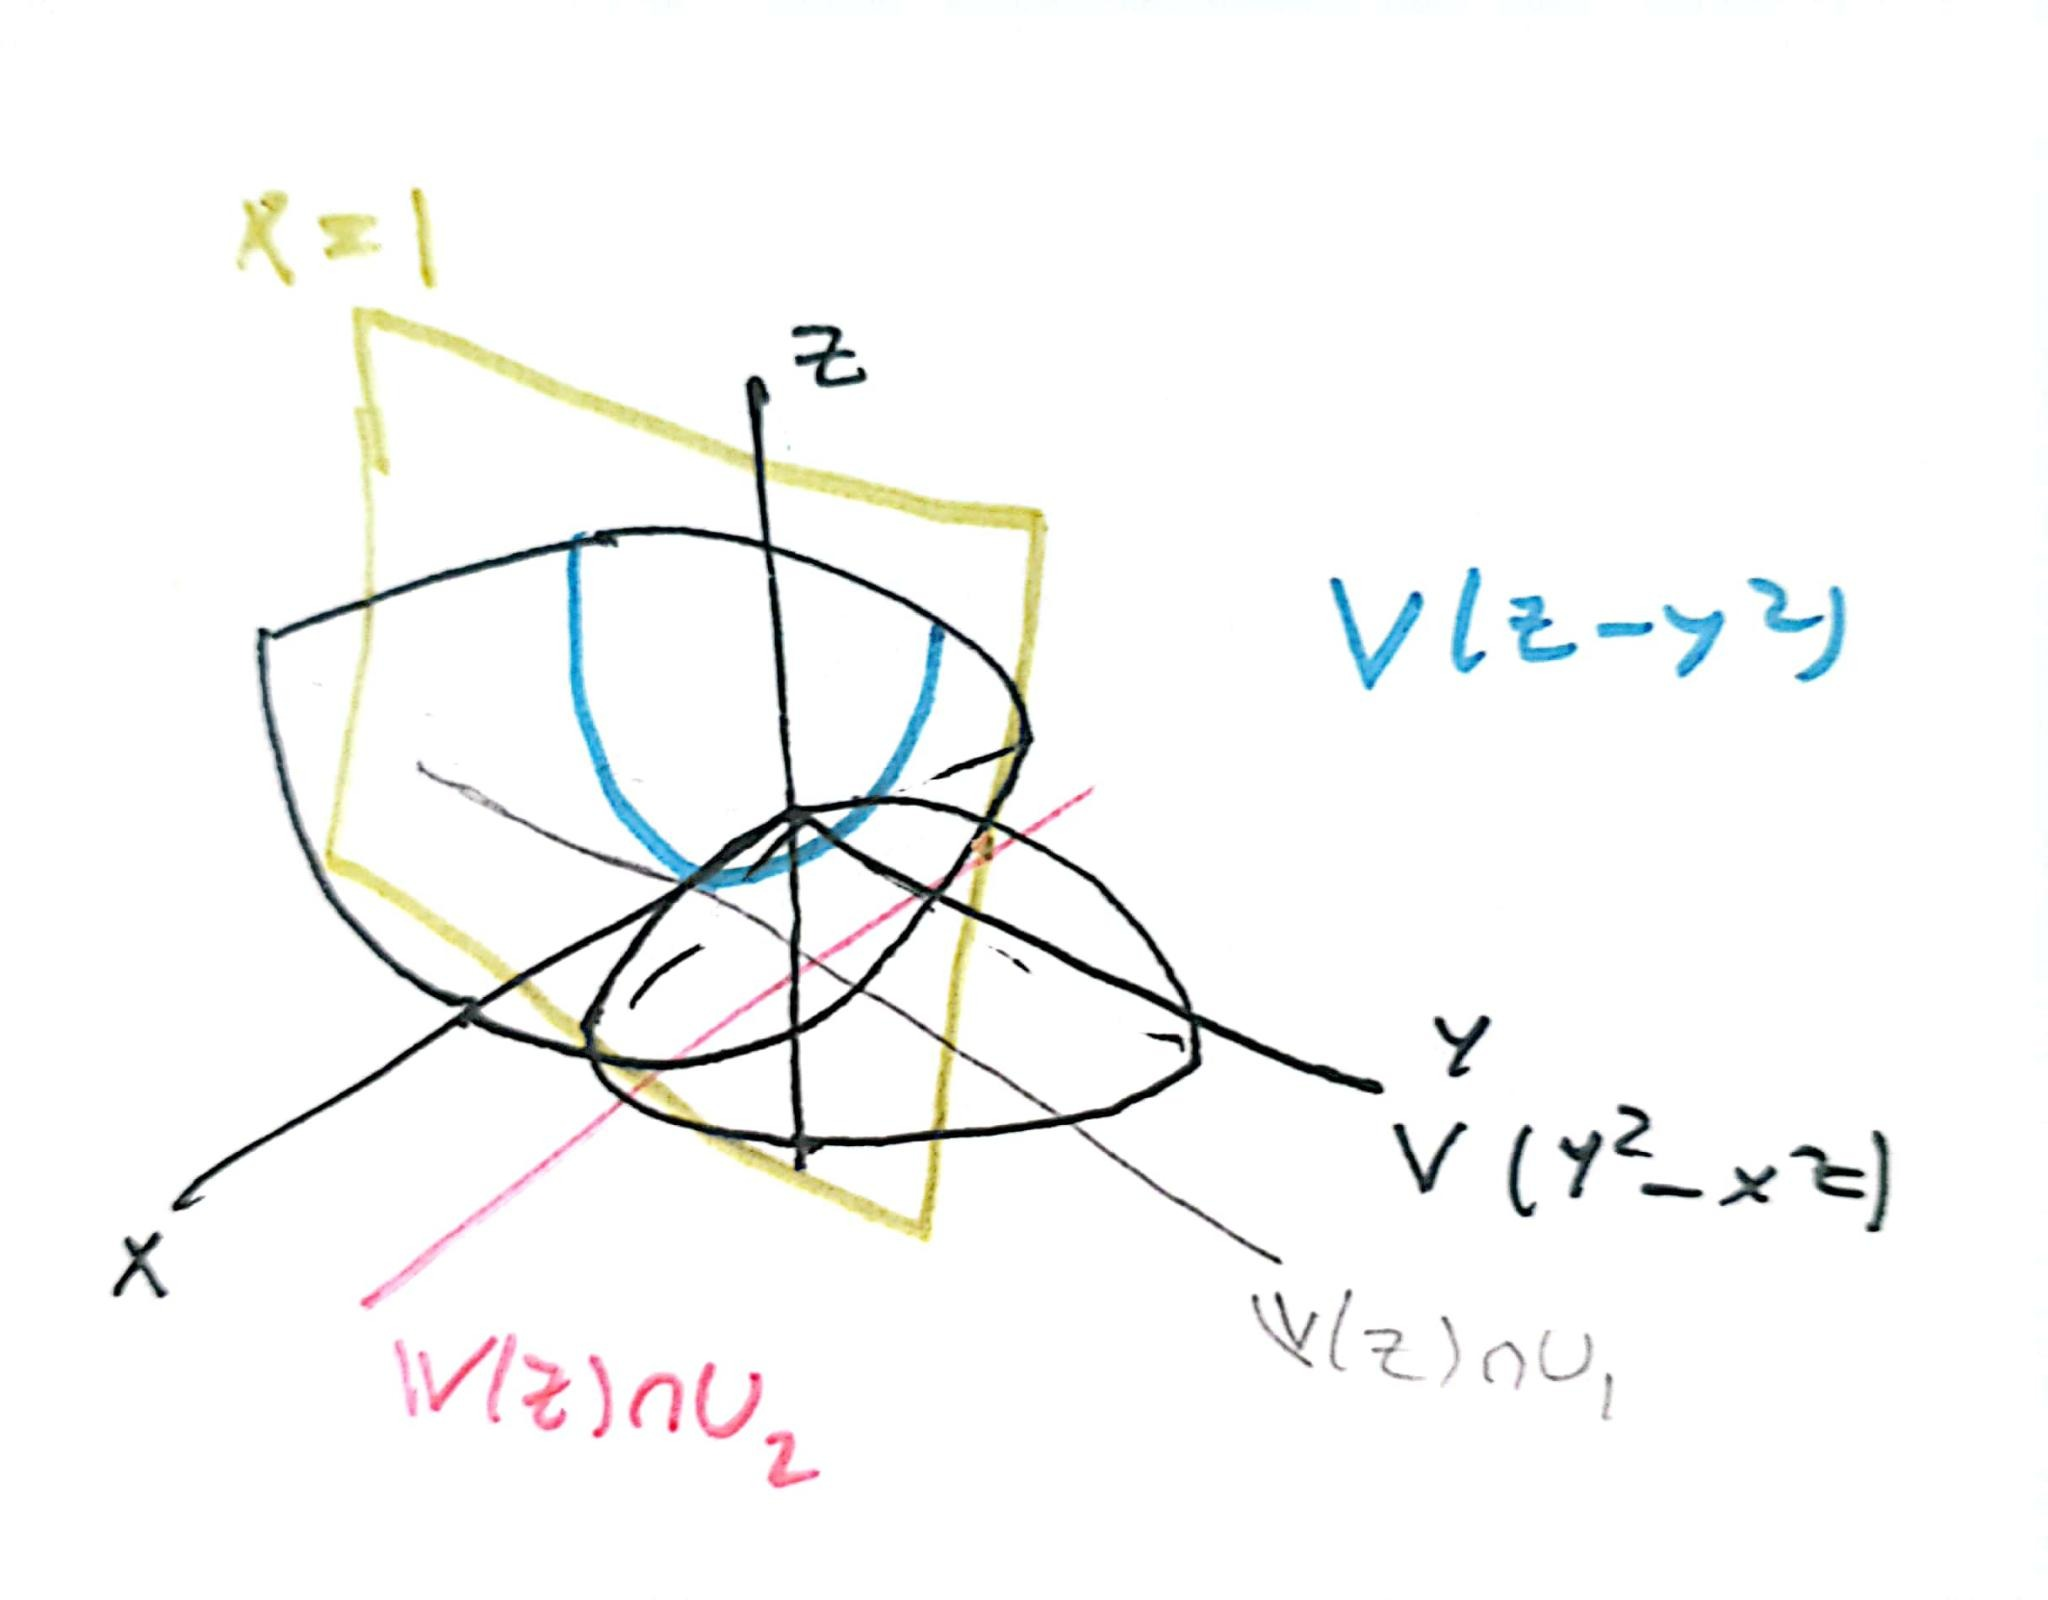
\includegraphics[width=0.8\textwidth]{3c4.jpeg}
       \label{fig:3c4-jpeg}
   \end{figure}
   
    
    
    
    
    
   \textbf{4:}\\
   (a) ($\implies$ ): Assume firstly that $I$ is prime. Let  $F,G \in k\left[ x_1, \ldots,
   x_{n+1} \right] $ be homogeneous. Assume $FG \in I$, then by assumption,
   $F \in I$ or $G \in I$.\\
   ($\Leftarrow$ ): Now assume conversely that for every pair of homogeneous
   polynomials $F$ and $G$, if $FG \in I$, then $F \in I$ or $G \in I$.\\
   Let now $f,g \in I$. Since $I$ is a homogeneous ideal in $k\left[ x_1,
   \ldots, x_{n+1}\right] $, we can write
   $I = \left( \left\{ F_{i} \right\}  \right) $ for homogeneous polynomials
   $F_i$. Thus we have
   $f = \sum F_{i_f}$ and $g = \sum F_{i_g}$. Hence
   \[
       fg = \sum \underbrace{F_{i_f} F_{i_g}}_{\in I} \in I
   \] 
   as $I$ is an ideal and thus closed under sums and multiplication.\\
   Therefore $I$ is a prime ideal.\\
   \linebreak
   (b) Suppose $f \in \sqrt{I} $. Then $f^{n} \in I$ for some $n$. Suppose
    $f = f_m + f_{m+1} + \ldots + f_d$ for some $0 \le m \le d$. Then
    the lowest degree term of $f^{n}$ is of degree $n \cdot m$ and is
    precisely $f_{m}^{n}$. As $I$ is a homogeneous polynomial, we have
    $f_{m}^{n} \in I$ by the last definition/proposition on lecture note 18,
    so in particular $f_m \in \sqrt{I} $. Now, as
    $\sqrt{I} $ is an ideal as was shown on HW2, we have $f - f_m \in \sqrt{I} $, which has
    lowest degree term of degree  $m+1$. Repeating this process 
     $d-m +1$ times, we find that
     $f_i \in \sqrt{I} $ for all $i \in \left\{ m, m+1, \ldots, d \right\} $,
     so
     by the last definition/proposition on lecture note 18, we find that
     $\sqrt{I} $ is homogeneous as $f\in \sqrt{I} $ was arbitrary.\\
     \linebreak
     \textbf{5:} Suppose $V(f) \subset \mathbb{A}_{\mathbb{R}}^2$ is
     a circle.\\
     We have that $V(f) \subset \mathbb{A}_{\mathbb{R}}^2$ is a circle
     if and only if $V(f) = 
     V\left( (x-a)^2 + (y-b)^2 - R^2 \right) $ which has
     corresponding subset in $\mathbb{P}^2$ and homogenization
     \[
     \left\{ \left[ x : y : 1 \right]  \colon 0 = y^2
     +a^2 - 2 a x + b^2 - 2 by - R^2 + x^2 \right\} 
     = \left\{ \left[ x : y : z \right]  \colon 0 = 
     y^2 + a^2 z^2 - 2axz + b^2 z^2 - 2byz - R^2 z^2 + x^2 \right\} 
     \] 
     So $F = y^2 + a^2 z^2 - 2axz + b^2 z^2 - 2byz - R^2 z^2 + x^2$.
     Now, letting $z = 0$, we find
     $y^2 +x^2 = 0$ which has solutions
     $\left[ 1 : i \right] $ and $\left[ 1 : -i \right] $ since
     $(1)^2 + (i)^2 = 1-1 = 0$ and $(1)^2 + (-i)^2 = 1-1 = 0$. Hence
     \[
     \left\{ \left[ 1: i :0 \right] , \left[ 1 : -i : 0 \right]  \right\} 
     \subset \mathbb{V} (F) \subset \mathbb{P}_{\mathbb{C}}^2
     \] 
     so $\mathbb{V}(F)$ meets the line at infinite in
     $\left\{ \left[ 1 : i : 0 \right] , \left[ 1: -i : 0 \right]  \right\}
     $.\\
     Furthermore, $V(f) \subset \mathbb{A}_{\mathbb{R}}^2$ is infinite
     since $(x-a)^2 + (y-b)^2 - \mathbb{R}^2$ has infinitely many roots over
     $\mathbb{R}^2$.\\
     \linebreak
     Conversely, suppose $\mathbb{V}(F) \subset \mathbb{P}_{\mathbb{C}}^2$ 
     meets
     the line at infinity in $\left\{ \left[ 1:i:0 \right] , \left[ 1:-i:0 \right]  \right\} $ 
     and $V(f) \subset \mathbb{A}_{\mathbb{R}}^2$ is infinite.\\
     \linebreak
     Write $f = ax^2 + by^2 + cxy + dx + ey + g$. We find that
     $F = ax^2 + by^2 + cxy + dxz + eyz + gz^2 \in \mathbb{R}\left[ x,y,z \right] 
     \subset \mathbb{C}\left[ x,y,z \right] $ is its homogenization of degree
     $2$.
     As $\mathbb{V}(F)$ meets
     the line at infinite at $\left\{ \left[ 1:i:0 \right] ,\left[ 1:-i:0
     \right]  \right\} $,
      we have $a - b + ic = 0$ and
      $a - b - ic = 0$, so $2 ic = 0$ gives $c = 0$. Hence
      $f = ax^2 + ay^2 + dx + ey + g$.
      Now $f (x,y) = 0$ if and only if
      $ax^2 + ay^2 + dx +ey + g = 0$ if and only if (as $f$ is of degree $2$,
      $a$ must be nonzero, so)
      $x^2 + y^2 + \frac{d}{a}x + \frac{e}{a}y + \frac{g}{a} = 0$ if and only
      if
      $$\left(\underbrace{x + \frac{d}{2a}}_{\in \mathbb{R}} \right)^2 + \left(
          \underbrace{y + \frac{e}{2a}}_{\in \mathbb{R}}
          \right)^2
      =  \frac{d^2}{4a^2} + \frac{e^2}{4a^2} - \frac{g}{a}.
       $$ Now, since $V(f) \subset \mathbb{A}_{\mathbb{R}}^2$ is
      infinite, we must have that
      $\frac{d^2}{4a^2} + \frac{e^2}{4a^2} - \frac{g}{a} >0$, and hence its
      square root exists, so we find that
      $f$ is precisely a circle with center $\left( -\frac{d}{2a},
      -\frac{e}{2a} \right) $ and radius
      $\sqrt{\frac{d^2}{4a^2} + \frac{e^2}{4a^2} - \frac{g}{a}} $.


   

    
    





















\end{document}
